% !TEX program = pdflatex
%
% Categorical foundations for general systems theory
% J. A. Goguen, IBM Thomas Watson Research Center, New York, USA
%
% Digitisation from a two-column scan: OCR was run column-by-column and
% then cleaned by hand. Figures are kept as image insertions taken from the
% original scan -- the cropped column PNGs live under columns/.
%
% Manual-review checklist:
%   * Compare each section against the corresponding column screenshots in
%     columns/page-NN-{01-left,02-right}.png.
%   * The mathematical symbols below are a *first pass*: OCR badly garbles
%     calligraphic letters and Greek glyphs, so every formula needs to be
%     re-checked against the scan. Suspect spots are flagged with TODO.
%   * Figures 1--12 are inserted as graphics placeholders -- crop them out
%     of the column screenshots when you have the chance and replace the
%     \missingfigure call with \includegraphics.

\documentclass[10pt,a4paper,twocolumn]{article}

\usepackage[T1]{fontenc}
\usepackage[utf8]{inputenc}
\usepackage[margin=2cm]{geometry}
\usepackage{amsmath, amssymb, amsthm}
\usepackage{mathrsfs}
\usepackage{graphicx}
\usepackage{xcolor}
\usepackage{hyperref}
\usepackage{quiver}
\usepackage{xspace}
\usepackage{float}
\usepackage{subcaption}

% Tighter inter-column gap and a thin rule between columns.
\setlength{\columnsep}{1.5em}

% --- Theorem environments -----------------------------------------------------
\newtheorem{theorem}{Theorem}
\newtheorem*{definition*}{Definition}

% --- Convenience macros -------------------------------------------------------
\newcommand{\A}{\mathcal{A}}          % a generic T-object (script A)
\newcommand{\B}{\mathcal{B}}         % a second T-object
\newcommand{\C}{\mathcal{C}}         % a third T-object
\newcommand{\Scal}{\mathcal{S}}
\newcommand{\X}{\mathcal{X}}
\newcommand{\Y}{\mathcal{Y}}
\newcommand{\Z}{\mathcal{Z}}
\newcommand{\W}{\mathcal{W}}
\newcommand{\CUR}{\underline{\textsc{cur}}\xspace}
\newcommand{\Ocat}{\mathbf{O}}          % arbitrary object category
\newcommand{\Tcat}{\Ocat_{T}}      % category of T-objects
\newcommand{\TcatS}[1]{\Ocat_{T,#1}}% T-objects over a given structure
\newcommand{\Scat}{\mathbf{S}}          % structure category
\newcommand{\Dcat}{\mathbf{D}}          % diagram category
\newcommand{\Rcal}{\mathcal{R}}          % a T-relation
\newcommand{\Iset}{\mathbf{I}}          % family of distinguished subsets
\newcommand{\R}{\mathbb{R}}
\newcommand{\Rpos}{\R^{+}}
\newcommand{\PF}{\mathrm{PF}}
\newcommand{\dom}{\mathrm{d}}            % "d f" = domain of f

% --- Original-page-number markers ---------------------------------------------
% \origpage{N} drops a small italic ``p.~N'' marker in the outer margin to
% indicate that page N of the original Goguen scan begins at this point in
% the text. Trim the margin-note geometry so the markers actually fit in
% the narrow 2cm outer margin of the two-column layout.
\setlength{\marginparwidth}{1.4cm}
\setlength{\marginparsep}{1.5mm}
\newcommand{\origpage}[1]{%
  \marginpar{\raggedright\footnotesize\itshape p.~#1}%
}


\title{Categorical foundations for general systems theory%
  \thanks{Digitised from a scan obtained by Matteo Capucci, with the help of Tesseract and Claude Opus 4.7 (for the initial pass, then manually checked and edited). OCR scripts available \href{https://github.com/mattecapu/goguen-categorical-foundations}{on GitHub}.}}
\author{J.\,A.~Goguen\\
        \small IBM Thomas Watson Research Center, New York, USA}
\date{}

\begin{document}
\maketitle


% =============================================================================
\section{Introduction}
% page-01 left + right
% =============================================================================

\origpage{121}%
There is a confusion of terminology which, if beyond our ability to dispel, merits some attention.
The phrase `general systems theory' often designates rather nonmathematical investigations in the philosophy and methodology of science.
By contrast, `linear systems theory' usually designates a well developed branch of engineering mathematics, now employing techniques such as Schwartz distribution theory (see~\cite{ZadehDesoer}). Between these is `mathematical systems theory' which tries to approach some problems of general systems theory through mathematical models.
As yet the technique of mathematical systems theory has not developed much beyond set theory. Mathematical systems theory is sometimes called general systems theory, and almost anything is called systems theory.
This may not be inappropriate, because almost anything can be viewed as a system.
In addition a distinction between formal and informal (possibly general) systems theories is sometimes made, parallel to the distinction between pure and applied mathematics.
Sometimes informalists oppose formalisms.

I believe categorical algebra can operate at the highest level of generality and still yield interesting results in systems theory.
Although some structure is necessary for interesting results, generality is achieved by treating structure as a parameter.
It seems that this theory is absolutely general systems theory, in the sense that I cannot imagine any system type which would not fit in its framework.
I believe other systems theories have difficulty with examples in Section~2, although these examples hardly
approach the potential of exotic systems.
While this work has not progressed far in a strictly practical direction, I think the relevance to philosophical and methodological questions will be clear.
Eventually applications to operating systems, state diagrams, Turing machines, and other information science basics should be included (linear systems and automata are discussed).
We hope that this material will be useful in explaining, organizing, and exploiting the many parallels between various disciplines.
The hierarchical structures of Section~6 should be useful for programming and biological systems.

% page-02 left
\origpage{122}%
Systems exhibit dynamic behavior; this is represented by a higher dimensional time-parameterized static system.
Our concept of system emphasizes `system theoretic' structures such as interconnection and level, rather than generalized automaton structures such as state and transition.

The content can be summarized as follows: $T$-objects model a collection of observations, and are in particular presheaves.
They motivate our constructions on a completely arbitrary category $\Ocat$ of \underline{objects}.
A \underline{system} is a diagram in $\Ocat$.
The \underline{behavior} of a system is its inverse limit.
Two systems are \underline{equivalent} if they have isomorphic behavior.
An \underline{interconnection} of systems is a direct limit in the category of diagrams.
Behavior and interconnections are pleasantly interrelated.
A hierarchical system structure results from considering higher order diagram categories.
There are several applications of the form: an interconnection of nice systems is nice.
Fuzzy systems are discussed.

It is necessary to assume some familiarity with categorical algebra; the
standard references are \cite{MacLane} and \cite{Mitchell}.
We do not use much more than the definitions of direct and inverse limit, natural
transformation, and presheaf.
We have omitted proofs.

This paper is more a program---that is, a reasonably well matched set of
methods and problems---than it is a finished work.
The completion of the program is a long-term project.
Our approach grew in part out of discussions with Hans Bremermann, Saunders MacLane, Christopher Longyear, Steve Soule, Victor Yngve, and Lofti Zadeh, all of whom we would like to thank.
The work is affectionately dedicated to the mysteries of human existence.

% =============================================================================
\section{\texorpdfstring{$T$-objects}{T-objects}}
% page-02 left tail + right + page-03 + page-04 left
% =============================================================================

This section is unnecessary for the general theory to follow, except as
motivation.
It is necessary for the applications of Sections~5 and~7 and is
of independent interest as an algebraic approach to epistemology and
entitation (see Quine~\cite{Quine}).

We formalize the notion of a collection of observations of an object.
Assume the observations parameterized over a space $T$, generally time.
$T$ might be the nonnegative reals $\Rpos$, or the nonnegative integers $\mathbb{N}$; choosing space-time as parameter, $T$ might be a submanifold of $\R^{4}$.
These examples suggest $T$ may have nontrivial structure, but for present purposes it suffices to assume $T$ is a set with a family $\Iset$ of distinguished subsets, usually some sort of intervals in~$T$.

If $X$ and $Y$ are sets, let $\PF[X,Y]$ denote the set of all partial functions from $X$ to $Y$, that is, functions to $Y$ from a subset of $X$, and let $\dom f$ denote the domain of $f\in\PF[X,Y]$.
Defining composition the obvious way with inverse image, there results a category of partial
morphisms of sets.
This construction can be duplicated in many categories.

\begin{definition*}
	A \emph{$T$-object} is a subset $\A$ of $\PF[T,A]$ such that $f\in\A \;\Rightarrow\; \dom f\in\Iset$; thus there is a domain map $\dom\colon \A\to\Iset$.
\end{definition*}

Here $A$ is some set of `attributes' over which our observations range.
We explicate the notion of object through the totality of potential parameterized observations of its attributes.
There is no need to posit ideal Platonic objects of which we gain imperfect knowledge through
observation, although there is need of abstraction and idealization in the construction of the totality from fragments of observations.
The detailed study of the manner of construction of objects from incomplete data belongs to the various sciences, but perhaps some useful generalities can emerge from the framework of this paper.
Now some examples of $T$-objects:

\begin{enumerate}
	\item \underline{A capacitor}.
	Suppose we control the voltage $v$ across a capacitor with a calibrated dial, and measure the resulting current $u$.
	Let $A=\R^{2}$, $T=\Rpos$, and $\Iset =$ the set of finite open intervals in $\Rpos$.
	Notice $f\in\PF[\Rpos,\R^{2}]$ can be viewed as a pair $\langle v,u\rangle$ of functions $\Rpos\to\R$ with the same domain.
	The collection of observations we might have gotten is
	\begin{equation*}
    \A = \left\{ \langle v,u\rangle \;\middle|\;
      \begin{aligned}
        & v,u\colon I\to\R \text{ differentiable}\\
        & \text{on } I\in\Iset,\ \text{and } u = \dot v
      \end{aligned}
    \right\}.
  \end{equation*}

	\item \underline{A finite state machine}.
	Suppose a machine has input alphabet $X$, output alphabet $Y$, state set $S$, state transition function $\lambda\colon X\times S\to S$, and output function $\delta\colon S\to Y$.
	Then $T$ is discrete time, starting at zero, i.e.\ $\mathbb{N}$, $\Iset$
	is the set of finite intervals in $\mathbb{N}$, and the set of
	observations\origpage{123} we might have collected is
	\begin{equation*}
    \A = \left\{
      \langle x,y\rangle
      \;\middle|\;
      \begin{aligned}
      & x\in\PF[\mathbb{N},X],\\
      & y\in\PF[\mathbb{N},Y],\\
      & \exists s\in\PF[\mathbb{N},S]\ \text{such that}\\
      & \dom x = \dom y = [n,m]\in\Iset,\\
      & \dom s = [n-1,m],\\
      & y(t) = \delta(s(t)),\\
      & s(t) = \lambda(x(t), s(t-1))\\
      & \text{for } t\in[n,m]
      \end{aligned}
    \right\}.
  \end{equation*}

	\item \underline{Temperature of a stone slab}.
	Suppose we observe the temperature of a stone as a time function over certain parts of its
	surface.
	Denote the surface $T$, a $3$-dimensional surface-time manifold in space-time $\R^{4}$.
  Then a temperature observation is a partial function $T\to\R$, with domain, say, an open set in $T$.
	The potential observations are the solutions of a certain partial differential equation.
  The purpose of this example is to show there are interesting $T$'s which are not merely semigroups, or simply ordered sets; so we omit distracting details.
\end{enumerate}

The set $A$ could also have relevant structure; it might be a product of sets of individual attributes; it might have a topological or differentiable structure which the functions in $\A$ respect; or perhaps an algebraic structure.
In example~1 the linear structure of $\R^{2}$ and the fact that the pairs $\langle v,u\rangle$ satisfy a linear relation give $\A$ a sort of linear structure.
In examples~1 and~3 the natural differentiable structures of $T$ and $A$ make the differentiability of the functions meaningful.
What concerns us most now is the resulting structure of $\A$, not how it arises; so we do not formalize these considerations, but pass on.

$\A$ can be viewed as an indexed family $\{\A_{I}\mid I\in\Iset\}$,
where
\begin{equation*}
  \A_{I} = \dom^{-1}I = \{\,f\in\A \mid \dom f = I\,\}.
\end{equation*}
This makes $\A$ a graded object of total functions, which is more convenient in many ways.
In example~1, each $\A_{I}$ is a real linear space of functions with total domain $I$.
From here on we assume each $\A_{I}$ is an object in a concrete category $\Scat$, called the
\emph{structure category}; so each $\A_{I}$ is in particular a set, and morphisms are in particular functions.

\begin{definition*}
	A \emph{morphism} $f\colon \A\to\B$ of $T$-objects is an indexed family $\{f_{I}\colon \A_{I}\to\B_{I}\}$ of $\Scat$-morphisms.
\end{definition*}

More abstractly, $f$ is a morphism of $\Iset$-graded objects of $\Scat$; less abstractly, $f$ is a function $f\colon \A\to\B$ which preserves domains (see Fig.~\ref{fig:tobj-morphism}) and $\forall I\in\Iset$ restricts to an $\Scat$-morphism $\A_{I}\to\B_{I}$.
Now some examples of morphisms.

\begin{figure}
	\begin{equation*}
		% https://q.uiver.app/#q=WzAsMyxbMCwwLCJcXEEiXSxbMiwwLCJcXEIiXSxbMSwxLCJcXEMiXSxbMCwyLCJcXGRvbSIsMl0sWzEsMiwiXFxkb20iXSxbMCwxLCJmIl1d
		\begin{tikzcd}
			\A && \B \\
			& \C
			\arrow["f", from=1-1, to=1-3]
			\arrow["\dom"', from=1-1, to=2-2]
			\arrow["\dom", from=1-3, to=2-2]
		\end{tikzcd}
	\end{equation*}
	\caption{\footnotesize $T$-object morphism.}%
	\label{fig:tobj-morphism}%
\end{figure}

\begin{enumerate}
	\item The above $\Rpos$-object containing observations on the capacitor has
	projections onto $\Rpos$-objects containing respectively voltage and
	current observations, defined by $\langle v,u\rangle\mapsto v$ and
	$\langle v,u\rangle\mapsto u$.
	These maps are continuous, differentiable, and linear.
	A linear change of scale for voltage measurement is described by a map of the form $\langle v,u\rangle\mapsto \langle\alpha v,u\rangle$ for $\alpha\in\R$.
  All such maps
	preserve domains.
	Nonlinear or discontinuous maps are conceivable, but not particularly appropriate.
	Here the structure category $\Scat$ is all real linear spaces, or better all linear topological spaces.
	Objects and maps of this general type are the subject matter of linear systems
	theory.

	\item For the finite state machine, the projections $\langle x,y\rangle \mapsto x$ and $\langle x,y\rangle\mapsto y$ define morphisms of $\mathbb{N}$-objects.
	More generally, changes of alphabet $f\colon X\to X'$, $g\colon Y\to Y'$ define morphisms $\langle x,y\rangle\mapsto \langle f(x),g(y)\rangle$, $\langle x,y\rangle\mapsto f(x)$, or $\langle x,y\rangle\mapsto g(y)$.
	Here $\Scat$ is the category of finite sets.
\end{enumerate}

The composition of two morphisms of $T$-objects, when defined, is a morphism of $T$-objects, and there results a category $\Tcat$ of all $T$-objects, to which we return in a moment.

$\Iset$ has a natural partial ordering (by inclusion) which makes it a category with at most one arrow in each $[I,J]$, the inclusion if $I\subseteq J$.
For objects arising in nature, we expect that if $f\in\A_{J}$ and $I\subseteq J$, then the restriction $f|_{I}\in\A_{I}$.
More formally, we expect $\A$ can be viewed as a functor $\A\colon \Iset^{\mathrm{op}}\to\Scat$ which maps the inclusion $I\subseteq J$ to the restriction map $\A_{J}\to\A_{I}$.
This means $\A$ is a \underline{presheaf of function}s; there is no general reason to suppose it a sheaf, though this can happen.

\origpage{124}%
Notice that the earlier view of a $T$-object as a graded object can also be
phrased as a presheaf, this time $\A\colon |\Iset|\to\Scat$.

\begin{definition*}
	A $T$-object $\A$ is \emph{closed under restriction}, abbreviated \CUR, iff it is a presheaf of functions; i.e.\ iff $I\subseteq J$ and $f\in\A_{J} \Rightarrow f\upharpoonright_{I}\in\A_{I}$.
\end{definition*}

$T$-objects closed under restriction form a subcategory of $\Tcat$; the morphisms are the natural transformations in the functor category $[\Iset,\Scat]$, families $\{f_{I}\mid I\in\Iset\}$ which commute with restriction.
See Fig.~\ref{fig:cur-morphism}.
It is clear then that $\Tcat$ is a full subcategory of $[|\Iset|,\Scat]$ (we will write $\Ocat_{T,\Scat}$ if we want to emphasize the role of $\Scat$) and \CUR $T$-objects form a full subcategory of $[\Iset,\Scat]$.
Actually, $\Tcat$ is equivalent to $[|\Iset|,\Scat]$ because we can always find an $\A$ such that $\A_{I} \cong \A'_{I}$, for any $\A'_{I}\in|\Scat|$, by choosing a large enough set $A$, and endowing appropriate sets of functions $I\to A$ with the $\Scat$ structure of $\A'_{I}$.

\begin{figure}
	\begin{equation*}
		% https://q.uiver.app/#q=WzAsNixbMCwwLCJKIl0sWzAsMSwiSSJdLFsyLDAsIlxcQV9KIl0sWzIsMSwiXFxBX0kiXSxbMywwLCJcXEJfSiJdLFszLDEsIlxcQl9JIl0sWzEsMCwiXFxzdWJzZXRlcSIsMl0sWzMsNSwiZl9JIiwyXSxbMiw0LCJmX0oiXSxbMiwzXSxbNCw1XV0=
		\begin{tikzcd}
			J && {\A_J} & {\B_J} \\
			I && {\A_I} & {\B_I}
			\arrow["{f_J}", from=1-3, to=1-4]
			\arrow[from=1-3, to=2-3]
			\arrow[from=1-4, to=2-4]
			\arrow["\subseteq"', from=2-1, to=1-1]
			\arrow["{f_I}"', from=2-3, to=2-4]
		\end{tikzcd}
	\end{equation*}
	\caption{\footnotesize \CUR morphism.}%
	\label{fig:cur-morphism}
\end{figure}

\begin{theorem}\label{thm:equivalence}
$\Ocat_{T,\Scat}$ is equivalent to $[|\Iset|,\Scat]$.
Similarly, the category of \CUR $T$-objects is equivalent to $[\Iset,\Scat]$.
\end{theorem}

For most purely categorical purposes, it suffices to know the category up to equivalence.
In particular, we have the following corollaries of Theorem~\ref{thm:equivalence}.

\begin{theorem}\label{thm:completeness}
If $\Scat$ is complete (or cocomplete, or finitely complete or cocomplete) so are $\Ocat_{T,\Scat}$ and the category of \CUR $T$-objects.
\end{theorem}

By \underline{complete}, we mean that every diagram has an (inverse) limit.
Recall the method of calculation of the (inverse) limit: it is the intersection of certain equalizers, as a subobject of the product of all the objects involved (see~\cite[p.~47]{Mitchell}); and for suitable concrete categories, it is the subobject of the (same) product consisting of all points whose coordinates form a `consistent net' under the mappings in the defining diagram.
This will be important for justifying our definition of behavior (see Section~4).

The notion of a $T$-object, with its arbitrary $T$ and $\Iset$, and associated structure category, is concrete, suggestive, and useful, though much more general than anything in the literature we know of.
It is closely related to ideas of Zadeh~\cite{ZadehDesoer}, Messarovi\'{c}~\cite{Messarovic}, and Windeknecht~\cite{Windeknecht}, from which we have drawn inspiration.
We believe it solves the problem of how to introduce specific structures conveniently into general systems theory.
However, systems of $T$-objects are more general, and the completely arbitrary systems of the next section are still more general.

% =============================================================================
\section{Systems}
% page-04 right tail + page-05 left + page-05 right (figures)
% =============================================================================

\origpage{125}%
\begin{figure}
  \begin{subfigure}{\linewidth}
    \centering
    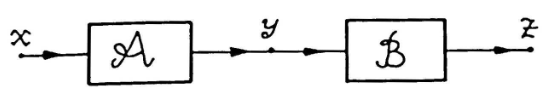
\includegraphics[width=.8\linewidth]{figures/fig3a.png}
    \caption{\footnotesize A graphical representation of a simple two-object system.}
    \label{fig:simple-system}%
  \end{subfigure}
  \begin{subfigure}{\linewidth}
    \centering
    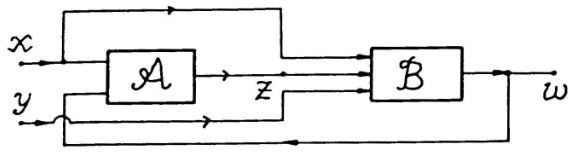
\includegraphics[width=.8\linewidth]{figures/fig3b.png}
    \caption{\footnotesize A graphical representation of a more complicated two-object system.}%
    \label{fig:two-object-system}%
  \end{subfigure}
  \caption{}
\end{figure}


\begin{definition*}
  A \underline{$\Tcat$-system} is a diagram in $\Tcat$, that is, a functor $S\colon D\to\Tcat$, where $D$ is called the index category or diagram \underline{scheme}.
\end{definition*}

The intended interpretation is: when two morphisms meet at an object, they shall display within that object identical representations of the objects at their domains.
The conventions and consequences of this interpretation can be developed without category theory; we hope the translation in Fig.~\ref{fig:diagram-3a-cat} of the graphs in Figs.~\ref{fig:simple-system} and~\ref{fig:two-object-system} suffice.

The formalization of the behavior of systems in the next section makes it explicit within our categorical framework.

We have introduced specific objects ($\X$, $\Y$, $\Z$, $\W$ in Fig.~\ref{fig:diagram-3a-cat}) to describe the allowed forms of flowing information; these are the \underline{domains} of the `system variables' ($x,y,z,w$ in Figs.~\ref{fig:simple-system} and~\ref{fig:two-object-system}), usually left implicit.

The definition of $T$-system depends in no essential way on properties of $T$-objects, although the intended interpretation does.
\underline{Absolute} generality can be achieved by replacing $\Tcat$ by an arbitrary, but preferably complete, category $\Ocat$ of suitable interconnectible objects, called \underline{objects}.

\begin{definition*}
  A \emph{system} is a diagram in $\Ocat$, that is, a functor $S\colon D\to\Ocat$, where $D$ is the index category or diagram scheme.
\end{definition*}

\begin{figure}
  \begin{subfigure}{\linewidth}
    \centering
    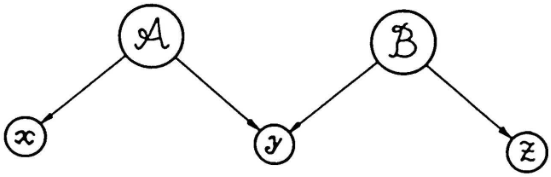
\includegraphics[width=.8\linewidth]{figures/fig4a.png}
    \caption{\footnotesize The categorical diagram for the system of Fig.~\ref{fig:simple-system}.
    Here the object $\A$ has projections of its interior states to an object $\X$ of inputs and an object $\Y$ of outputs, while $\B$ has projections to $\Y$ as inputs and $\Z$ as outputs.
    It is intended that the outputs of $\A$ be constrained to equal the inputs of $\B$, as points in $\Y$.}%
    \label{fig:diagram-3a-cat}%
  \end{subfigure}
  \begin{subfigure}{\linewidth}
    \centering
    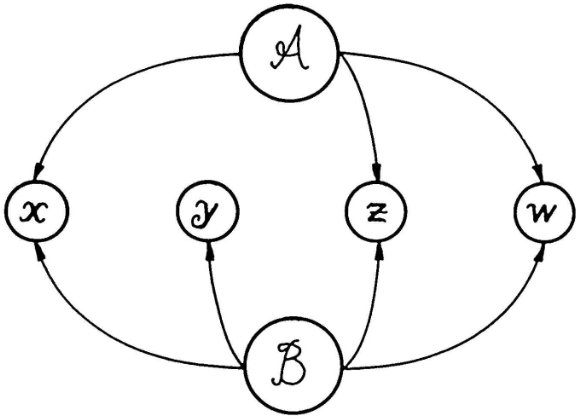
\includegraphics[width=.65\linewidth]{figures/fig4b.png}
    \caption{\footnotesize The categorical diagram for the system of Fig.~\ref{fig:two-object-system}.}%
    \label{fig:diagram-3b-cat}%
  \end{subfigure}
  \caption{}
\end{figure}


\begin{figure}
  \begin{equation*}
    \large
    % https://q.uiver.app/#q=WzAsMyxbMCwwLCJEIl0sWzIsMCwiRCciXSxbMSwxLCJcXE9jYXQiXSxbMCwyLCJTIiwyXSxbMSwyLCJTJyJdLFswLDEsIkYiXSxbMSwzLCJcXGV0YSIsMix7Im9mZnNldCI6LTIsInNob3J0ZW4iOnsic291cmNlIjozMCwidGFyZ2V0IjoyMH19XV0=
    \begin{tikzcd}
      D && {D'} \\
      & \Ocat
      \arrow["F", from=1-1, to=1-3]
      \arrow[""{name=0, anchor=center, inner sep=0}, "S"', from=1-1, to=2-2]
      \arrow["{S'}", from=1-3, to=2-2]
      \arrow["\eta"', shift left=2, between={0.3}{0.8}, Rightarrow, from=1-3, to=0]
    \end{tikzcd}
  \end{equation*}
  \caption{\footnotesize A system morphism.}%
  \label{fig:system-morphism}%
\end{figure}

\origpage{126}%
To model one system by or in another, we want morphisms of diagrams, and a category of diagrams (or systems) in $\Ocat$.

\begin{definition*}
  A \emph{morphism} from ${S\colon D\to\Ocat}$ to ${S'\colon D'\to\Ocat}$ is a pair $\langle F,\eta\rangle$, where $F\colon D\to D'$ is a functor and $\eta\colon S'F\to S$ is a natural transformation.
  See Fig.~\ref{fig:system-morphism}.
\end{definition*}

Denote by $\Dcat(\Ocat)$ the category of diagrams in $\Ocat$ with these morphisms.
This category is similar to the category of fuzzy sets with
values in $\Ocat$~\cite{GoguenVsets}, except the transformation $\eta$ goes the opposite way.

\begin{theorem}\label{thm:dcat-complete}
  $\Dcat(\Ocat)$ is cocomplete (or complete or finitely cocomplete or complete) if $\Ocat$ is complete (or cocomplete, or finitely complete or cocomplete).
\end{theorem}

% =============================================================================
\section{Behavior of systems}
% page-06 left tail + page-06 right + page-07 left + page-07 right
% =============================================================================

We want to know of a system how it behaves as an object when hooked up and let run.
We develop the concept through examples in $\Tcat$.
For simplicity, assume the structure category is $\mathbf{Ens}$, the category of sets.
\begin{figure}
  \begin{subfigure}{\linewidth}
    \centering
    
\includegraphics[width=.8\linewidth]{figures/fig6a.png}
    \caption{\footnotesize A system of two independent objects $\A$ and $\B$.}%
    \label{fig:indep-system}%
  \end{subfigure}
  \begin{subfigure}{\linewidth}
    \centering
    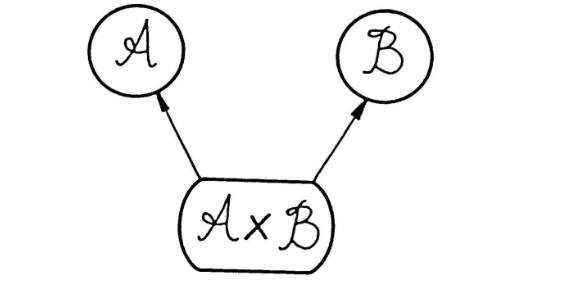
\includegraphics[width=.8\linewidth]{figures/fig6b.png}
    \caption{\footnotesize The system of Fig.~\ref{fig:indep-system} with its behaviour and projections.}%
    \label{fig:indep-behavior}%
  \end{subfigure}
  \caption{}
\end{figure}

\begin{enumerate}
  \item The first nontrivial case is two completely independent observations, represented by objects $\A$ and $\B$ (see Fig.~\ref{fig:indep-system}).
  Because we have no knowledge of which observations in $\A$ are paired with observations in $\B$ (if any), as far as we know, all pairings are possible, and the behavior of the system is described by $\A\times\B$.
  This with its projections to $\A$ and $\B$ forms a larger system (see  Fig.~\ref{fig:indep-behavior}).

  \item The next interesting case is two simultaneous observations.
  Here one has objects for the two observables, and another for observations of the pairing or simultaneity.
  This object $\Rcal$ consists of just those pairs which occur together.
  See Fig.~\ref{fig:simul-system}.
  There are projections from $\Rcal$, giving the components of the pairs.
  The behavior is clearly described already by $\Rcal$.

  \begin{figure}
    \centering
    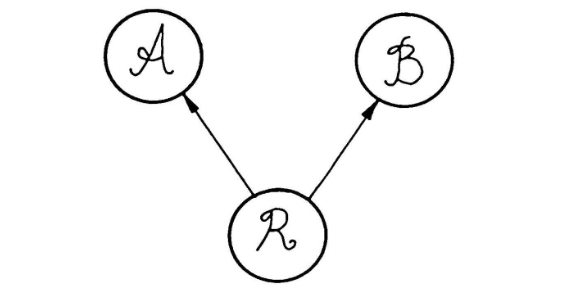
\includegraphics[width=.8\linewidth]{figures/fig7.png}
    \caption{\footnotesize Two simultaneous observation system.}%
    \label{fig:simul-system}%
  \end{figure}

  \origpage{127}%
  \begin{figure}
    \begin{subfigure}{\linewidth}
      \centering
      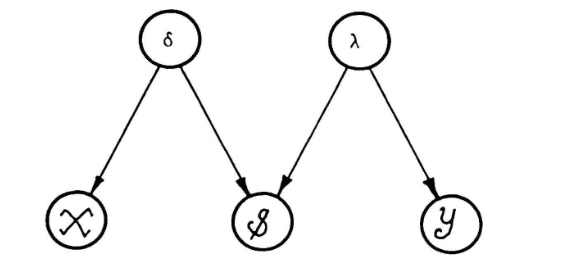
\includegraphics[width=.8\linewidth]{figures/fig8a.png}
      \caption{\footnotesize Finite state machine system diagram.}%
      \label{fig:fsm-diagram}%
    \end{subfigure}
    \begin{subfigure}{\linewidth}
      \centering
      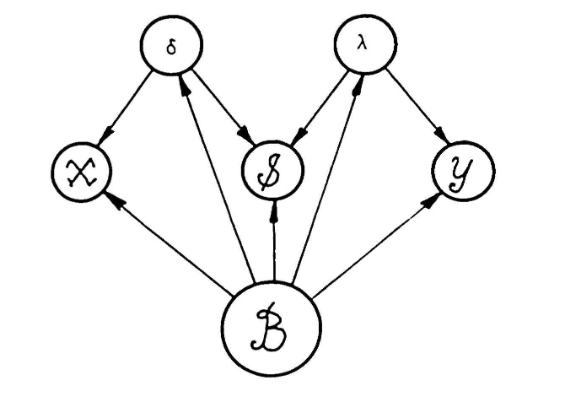
\includegraphics[width=.8\linewidth]{figures/fig8b.png}
      \caption{\footnotesize Behaviour of Fig.~\ref{fig:fsm-diagram}.}%
      \label{fig:fsm-behavior}%
    \end{subfigure}
    \caption{}
  \end{figure}

  \item A finite state machine can be represented by a system diagram like that in Fig.~\ref{fig:fsm-diagram}.
  $\X$ and $\Y$ are the objects of input and output observations, $\Scal$ is the object of state observations, and
  $\delta$ and $\lambda$ are respectively the objects for the state transition and output functions.
  $\Tcat$ is $\mathbb{N}$.
  The behavior will be those input-state-output triples which can occur for these $\delta$ and $\lambda$.
  Actually, $\delta$ and $\lambda$ give, respectively, those input-state and state-output pairs of observations (as functions of time, remember) which can occur, together with projections to the components which do occur.
  In this same spirit $\B$ is the object of triples, together with projections to pairs and to individuals.
  See Fig.~\ref{fig:fsm-behavior}.
  The structure category is finite sets; notice it is only finitely complete.
\end{enumerate}

In each case, the behavior is the (inverse) limit of the system diagram with the natural projections.
The interpretation of the diagrams (Section~3) together with the remarks on the calculation of the limit following Theorem~\ref{thm:completeness} (Section~2) show that this is true in general: the limit picks out just those tuples of mutually consistent observations among the system's objects.

\begin{definition*}
  The \emph{behavior} of $S\in\Dcat(\Ocat)$ is $\varprojlim S\in\Ocat$.
\end{definition*}

We have returned to the general case where $\Ocat$ is an arbitrary (preferably complete) category.
Notice behavior is a contravariant
functor,
\begin{equation*}
  \varprojlim\colon \Dcat(\Ocat)^{\mathrm{op}}\longrightarrow \Ocat,
\end{equation*}
because morphisms in $\Dcat(\Ocat)$ were defined appropriately.
In particular, behavior restricts to a functor
$\varprojlim\colon [D,\Ocat]^{\mathrm{op}}\to\Ocat$, for each diagram
scheme $D$, which commutes with limits, for example products, because it is an adjoint functor.

\begin{definition*}
  Systems $S,S'\in\Dcat(\Ocat)$ are \emph{equivalent} if they have isomorphic behavior.
\end{definition*}

Consider the hypothesis that some observed behavior (say example~2, i.e.\ Fig.~\ref{fig:simul-system}) came from a finite state machine (say example~3, Fig.~\ref{fig:fsm-diagram}).
Technically, the hypothesis is that the behaviors are isomorphic, i.e.\ the systems equivalent.
The inclusion of the diagram of Fig.~\ref{fig:simul-system} in that of Fig.~\ref{fig:fsm-behavior} induces a morphism of their limits (the limit of Fig.~\ref{fig:fsm-behavior} is just $B$ again), in the opposite direction.
The hypothesis is that this is an isomorphism.

Another application is in showing that a system whose objects have some property also has that property.
For example, is a system of linear objects linear?
The method is to show the (sub-)category of objects with that property is complete (finite completeness may be appropriate for examples such as~3); then the behavior is in the category.
It suffices to check products and equalizers, which is often easy.
A generalization of this application is discussed in more detail in Section~7.

% =============================================================================
\section{\texorpdfstring{$T$-relations}{T-relations}}
% page-07 right tail + page-08 left
% =============================================================================

A particularly interesting special case is diagrams of $T$-objects like Fig.~\ref{fig:simul-system}, with the additional restriction that $\Rcal$ be a subobject of $\A\times\B$ such that the projections commute;
i.e.\ the maps from $\Rcal$ to $\X$ and $Y$ are restrictions of the projections from $\X\times Y$ to $\X$ and $Y$ (respectively).
See Fig.~\ref{fig:t-relation}.
Call such a system a \underline{$T$-relation}.

\begin{figure}
  \begin{equation*}
    % https://q.uiver.app/#q=WzAsNCxbMCwyLCJcXFgiXSxbMiwyLCJcXFkiXSxbMSwxLCJcXFJyZWwiXSxbMSwwLCJcXFggXFx0aW1lcyBcXFkiXSxbMywwLCIiLDAseyJvZmZzZXQiOjJ9XSxbMywxLCIiLDIseyJvZmZzZXQiOi0yfV0sWzIsMywiIiwyLHsic3R5bGUiOnsidGFpbCI6eyJuYW1lIjoibW9ubyJ9fX1dLFsyLDBdLFsyLDFdXQ==
    \begin{tikzcd}
      & {\X \times \Y} & \\
      & \Rcal \\
      \X && \Y
      \arrow[shift right=2, from=1-2, to=3-1]
      \arrow[shift left=2, from=1-2, to=3-3]
      \arrow[tail, from=2-2, to=1-2]
      \arrow[from=2-2, to=3-1]
      \arrow[from=2-2, to=3-3]
    \end{tikzcd}
  \end{equation*}
  \caption{\footnotesize A $T$-relation $\Rcal$.}%
  \label{fig:t-relation}%
\end{figure}
\origpage{128}%
Its behavior is $\Rcal$.
$T$-relations form a category with the morphisms described in Section~3, but more interestingly $T$-relations can be made the morphisms of a category whose objects are $T$-objects, by defining the
composition of $\X \leftarrow \Rcal \to \Y$ and $\Y \leftarrow \Scal \to \Z$ to be the behavior of the interconnection (see Fig.~\ref{fig:t-rel-comp}), with projections to the terminals $\X$ and $\Z$.

\begin{figure}
  \begin{equation*}
    % https://q.uiver.app/#q=WzAsNixbMCwxLCJcXFgiXSxbMiwxLCJcXFkiXSxbMSwwLCJcXFJzY3IiXSxbMywwLCJcXFNzY3IiXSxbNCwxLCJcXFoiXSxbMiwyLCJcXFNzY3IgXFxjaXJjIFxcUnNjciJdLFsyLDBdLFsyLDFdLFszLDFdLFszLDRdLFs1LDBdLFs1LDRdXQ==
    \begin{tikzcd}
      & \Rcal && \Scal & \\
      \X && \Y && \Z \\
      && {\Scal \circ \Rcal}
      \arrow[from=1-2, to=2-1]
      \arrow[from=1-2, to=2-3]
      \arrow[from=1-4, to=2-3]
      \arrow[from=1-4, to=2-5]
      \arrow[from=3-3, to=2-1]
      \arrow[from=3-3, to=2-5]
    \end{tikzcd}
  \end{equation*}
  \caption{\footnotesize The composition of $T$-relations.}%
  \label{fig:t-rel-comp}%
\end{figure}

So $\Rcal'\circ\Rcal$ is a subobject of $\X\times \Z$, and
$\X \leftarrow \Scal \circ \Rcal \to \Z$ is a $T$-relation.

This category of $T$-relations has products: the product of $\X$ and $\Y$ is the coproduct (disjoint union) in $\Tcat$; a product of morphisms is also a coproduct in $\Tcat$, in the sense that $\Rcal \sqcap \Rcal'$ as an object is $\Rcal \sqcup \Rcal'$ in $\Tcat$.

% =============================================================================
\section{Interconnection of systems}
% page-08 left tail + page-08 right + page-09 left
% =============================================================================

If general systems theory is `about' anything, it is about the interconnection of systems, and the resulting behavior.
The manipulations of the previous section give some indication of the importance of these considerations.
The very general results of this section are the core of this paper.

If two systems (diagrams in $\Ocat$) have a common subsystem, we can form their `union' or interconnection.
Different systems may result from the same two systems by specifying different subdiagrams as common.
The common subdiagram is often a collection of objects at terminals hooked together.
The restriction to two systems is inessential.
The proper formalization is the \underline{direct limit} of diagrams.
But not every diagram of diagrams can arise.

\begin{definition*}
  An \underline{interconnection} is a diagram $S\colon X \to \Dcat(\Ocat)$, all morphisms $\langle I,\eta\rangle$ of which consist of an inclusion $I$ of diagram schemes, and have monic values $\eta_{\X}$ of the transformation $\eta$.
  Denote the subcategory of $\Dcat(\Ocat)$ with morphisms as described above by $\Dcat_{0}(\Ocat)$, and call it the \underline{interconnection category}.
  Properties of $\Dcat_{0}(\Ocat)$ or some close relative should be worthy of future study.
\end{definition*}

We speak of an interconnection $S$ of systems $S_{\X}$, $\X\in|X|$.

\begin{definition*}
  The direct limit in $\Dcat(\Ocat)$ of a diagram $S$ of diagrams will be the \underline{result} of $S$.
\end{definition*}

\begin{theorem}\label{thm:interconnect}
  If $\Ocat$ has intersections and inverse images, any interconnection has a result.
\end{theorem}

So systems of reasonable objects are always interconnectable.
For example, let $S_{1}$ and $S_{2}$ be systems, interconnected with no common objects or morphisms.
The result is the coproduct, $S_{1}\sqcup S_{2}$, whose diagram is the disjoint union of those of $S_{1}$ and $S_{2}$.
See Fig.~\ref{fig:disjoint-union}.
A more specific example appears in Fig.~\ref{fig:specific-interconnect}.

\begin{figure}
  \begin{subfigure}{\linewidth}
    \begin{equation*}
      % https://q.uiver.app/#q=WzAsMixbMCwwLCJTXzEiXSxbMiwwLCJTXzIiXV0=
      \begin{tikzcd}
        {S_1} && {S_2}
      \end{tikzcd}
    \end{equation*}
    \caption{\footnotesize Disjoint union diagram for two systems $S_{1}$ and $S_{2}$.}
    \label{fig:disjoint-union-a}
  \end{subfigure}
  \begin{subfigure}{\linewidth}
    \begin{equation*}
      % https://q.uiver.app/#q=WzAsMyxbMCwwLCJTXzEiXSxbMiwwLCJTXzIiXSxbMSwxLCJTXzEgXFxzcWN1cCBTXzIiXSxbMSwyXSxbMCwyXV0=
      \begin{tikzcd}
        {S_1} && {S_2} \\
        & {S_1 \sqcup S_2}
        \arrow[from=1-1, to=2-2]
        \arrow[from=1-3, to=2-2]
      \end{tikzcd}
    \end{equation*}
    \caption{Result of the interconnection of \ref{fig:disjoint-union-a} with inclusions.}
  \end{subfigure}
  \caption{}
  \label{fig:disjoint-union}
\end{figure}

\begin{figure}
  \begin{subfigure}{\linewidth}
    \centering
    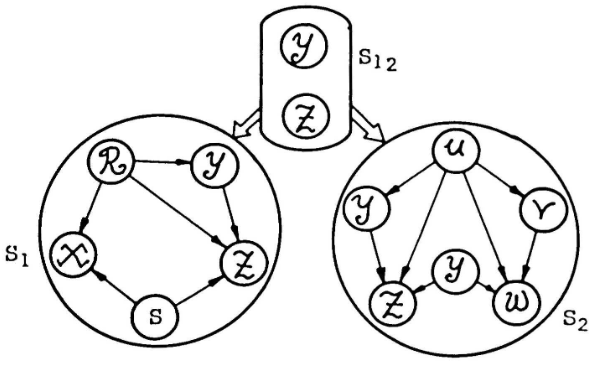
\includegraphics[width=.8\linewidth]{figures/fig12a.png}
    \caption{\footnotesize An interconnection of $S_{1}$ and $S_{2}$ with common subsystem
     $S_{12}$.}%
    \label{fig:specific-interconnect}%
  \end{subfigure}
  \begin{subfigure}{\linewidth}
    \centering
    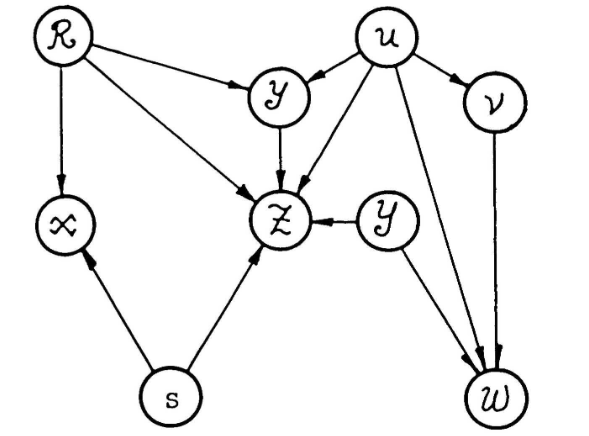
\includegraphics[width=.8\linewidth]{figures/fig12b.png}
    \caption{\footnotesize Result of the interconnection.}%
    \label{fig:specific-interconnect-result}%
  \end{subfigure}
  \caption{}
\end{figure}

\origpage{129}%
The \underline{behavior} of an interconnection of systems is the (inverse) limit of the result.
Two interconnections are \underline{equivalent} if they have isomorphic behavior.

It is important to calculate the behavior of an interconnection from the behaviors of its component systems.
The result below shows how.

\begin{theorem}\label{thm:lim-of-lim}
  Let $S\colon X \to \Dcat(\Ocat)$ be an interconnection of systems $S_x\colon D_x \to \Ocat$, for $x \in X$.
  Then
  \begin{equation*}
    \varprojlim\bigl(\varinjlim S\bigr) \;=\;
    \varprojlim_x\bigl(\varprojlim S_x\bigr).
  \end{equation*}
\end{theorem}

The right-hand side is the (inverse) limit of the diagram of behaviors of systems $S_x$, whose morphisms are those induced on the behaviors by the morphisms $x$ of $\X$.
The left-hand side is just the definition of the behavior of the interconnection.
The Theorem says how to compute it from the $\varprojlim S_x$'s.

One can obtain various canonical forms for systems.
For example, every system is equivalent to an interconnection of subsystems with (at most) two objects and one morphism.
By adding some objects, the number of morphisms at (meaning either to or from) each object in the equivalent system can be made three or less.
If $\Ocat$ is `normal', the morphisms can be restricted to monics and epics, by adding images.

The considerations of this section can be extended hierarchically by
letting $\Ocat$ be $\Dcat(\Ocat)$, or more generally, defining
\begin{equation*}
  \Dcat^{n}(\Ocat) = \Dcat\,\Dcat^{n-1}(\Ocat), \qquad
  \Dcat^{0}(\Ocat) = \Ocat.
\end{equation*}
Theorems~\ref{thm:interconnect} and~\ref{thm:lim-of-lim} apply at any level.
It should be useful to consider the category
\begin{equation*}
  \Dcat^{\infty}(\Ocat) \;=\; \varinjlim_{n} \Dcat^{n}(\Ocat),
\end{equation*}
the limit being in $\mathbf{Cat}$.
Similarly we can form $\Dcat_{0}^{n}(\Ocat)$ and $\Dcat_{0}^{\infty}(\Ocat)$.
We believe these categories will be useful in studying programming languages or other hierarchically organized systems.
The functor $\varprojlim$ extends to the direct limits $\Dcat^{n}(\Ocat)$ or $\Dcat^{\infty}(\Ocat)$.

% =============================================================================
\section{Applications}
% page-09 right + page-10 left + page-10 right
% =============================================================================

Our first applications have the form: an interconnection of systems of type $T$ is type $T$.
This is proved by showing the category of type $T$ objects is complete.
It follows that systems, and results of interconnections, have type $T$ behavior.
There is really no need for all objects to be type $T$ as long as each system has type $T$ behavior.
Our categorical machinery effects a great simplification for such problems.
Now some examples; we refer to Section~2 for background.

\begin{enumerate}
  \item An interconnection of linear systems is linear.
  A general setting for this result is as follows: let $\Iset$ be a fixed category (think of intervals in some $T$, partially ordered by inclusion), and let $\Scat$ be $\mathbf{Lin}$, the category of linear spaces, say over $\R$.
  Let $\Ocat$ be the functor category $[\Iset,\mathbf{Lin}]$.
  It is complete because $\mathbf{Lin}$ is.
  More concretely one could consider $\Ocat_{T,\mathbf{Lin}}$ for some particular $T$.

  \item An interconnection of continuous systems is continuous.
  Proceeding as above, let $\Scat$ be $\mathbf{Top}$, the category of topological spaces.
  Then $[\Iset,\mathbf{Top}]$ is complete.

  \item An interconnection of differentiable systems is differentiable.
  Consider the (complete) category of differentiable manifolds.

  \item An interconnection of invariant systems is invariant.
  Let $G$ be a semigroup of endomorphisms of $T$ such that the induced map on subsets restricts to an endomorphism of $\Iset$.
  Let $\Iset_{0}$ be a subset of $\Iset$ of distinguished intervals, for example, in $\Rpos$, those of the form $(0,t)$.
  Then a $T$-object is \underline{$G$-invariant} iff each $\A_{I}$ is of the form $g\,\A_{J}$, some $g\in G$ and $J\in\Iset_{0}$, where $g\,\A_{J} = \{f\circ g \colon g(J)\to A \mid f\in\A_{J}\}$.
  The first examples which come to mind are\origpage{130} translations: if $T=\mathbb{N}$, then $G=\mathbb{N}$ and $g(t)=g+t$, for $g\in G$ and $t\in T$.
  It suffices to check products and equalizers, and these are essentially obvious.

  \item An interconnection of $T$-relations is equivalent to a $T$-relation.
  This application is of a different character from these previous because \underline{equivalence} is asserted and the properties in question are \underline{system} properties not derived from object properties.
  The notions of interconnection and equivalence here also differ from those given earlier.

  \begin{definition*}
    Let $S\colon D\to\Ocat$ and let $D_{0}\subseteq D$.
    Then the \underline{behavior of $S$ modulo $D_{0}$} is $\varprojlim S$ together with its projections to objects in $D_{0}$.
    It is a diagram, in fact a cone over $D_{0}$, in $\Ocat$.
  \end{definition*}

  \begin{definition*}
    Let $S_{i}\colon D_{i}\to\Ocat$, $i=1,2$ be systems and let $D_{12}$ be
    embedded in $D_{1}$ and $D_{2}$.
    Then $S_{1}$ and $S_{2}$ are \emph{equivalent modulo $D_{12}$} (and the embeddings) iff they have isomorphic (in $\Dcat(\Ocat)$) behaviors modulo $D_{12}$.
  \end{definition*}

  The diagram subscheme appropriate for $T$-relations is $\mathbf{2}$, the two point discrete category.

  \item An interconnection of causal $T$-relations is causal.
  Let $\delta\colon \Iset\to 2^{T}$ be a boundary or successor operator on subsets of $T$.
  If $\A \leftarrow \Rcal \to \B$ is the graph of a morphism in $\Tcat$, call it \underline{causal} if
  \begin{align*}
    & f = \langle u,v\rangle,\ f' = \langle u',v'\rangle \in \Iset,\\
    & \dom f = \dom f' = I\in\Iset,\\
    & J\in\Iset,\ \theta J\subseteq I,\\
    & f\upharpoonleft J = f' \upharpoonright J = f \upharpoonright \theta J = f' \upharpoonright \theta J.
  \end{align*}
  An arbitrary $T$-relation $\A\to\Rcal\to\B$ is causal iff it is a union of causal sub-$T$-relations which are graphs of morphisms in $\Tcat$.
  This definition is based on Windeknecht~\cite{Windeknecht}.

  \item Fuzzy systems.
  Let $V$ be a complete lattice, and let $\mathcal{S}(V)$ be the category of \emph{$V$-sets}, whose objects are functions $X\to V$, where $X$ is a set, and whose morphisms $A \to B$ are functions $f\colon X\to Y$ such that $A(x) \leq B(f(x))$ for all $x\in X$; this category is complete and rather like the category of sets (see~\cite{GoguenLfuzzy} or~\cite{GoguenVsets} for more details).
  $\mathcal{S}(V)$ is not concrete as defined, but it is isomorphic (not just equivalent) to the concrete category whose object corresponding to $\A\colon X\to V$ is the subset of $X\times V$ of points less than or equal to (in the product ordering of $\prod_{x \in X} V_x$ [sic]) the graph of $\A$, and whose morphisms arise similarly from those of $\mathcal{S}(V)$.
  If $\Ocat$ is the category of $T$-systems with structure $\mathcal{S}(V)$, then $\Dcat(\Ocat)$ is the category of \emph{fuzzy systems}.
  It has been argued~\cite{GoguenLfuzzy,GoguenInexact} that $V$-sets represent inexact concepts and are the building blocks of inexact structures; it has also been argued~\cite{ZadehFuzzy} that fuzzy systems of various sorts (including fuzzy algorithms~\cite{ZadehAlgorithms}) are important for understanding such pervasive phenomena as optimization in an inexact environment.
  Our notion of fuzzy system, including the hierarchies of system structure and arbitrary $T$ and $\Iset$, is much more general than anything we know in the literature.
  And we hope more applicable, because it is more structured.
  For example, fuzzy systems can probably model word association nets of the sort metaphorically described by Quine~\cite{Quine}, p.~12.
  Contemplate
  \begin{equation*}
    D^\infty_0\left(\Ocat_{\mathbf{N}, \mathcal{S}([0,1)}\right).
  \end{equation*}
\end{enumerate}


% =============================================================================
\section*{Bibliography}
% page-10 right
% =============================================================================

\begin{thebibliography}{12}

\bibitem{GoguenLfuzzy}
J.~A.~Goguen, `L-fuzzy sets',
\emph{J.~Math.\ Analysis Applic.}, \textbf{18}(1), pp.~145--174 (April 1967).
\href{https://doi.org/10.1016/0022-247X(67)90189-8}%
     {\nolinkurl{doi:10.1016/0022-247X(67)90189-8}}.

\bibitem{GoguenInexact}
J.~A.~Goguen, `The logic of inexact concepts',
\emph{Synthese}, \textbf{19}(3--4), pp.~325--373 (1969).%
\footnote{The original paper lists the page range as ``pp.~1--48''; the
  correct range in \emph{Synthese} \textbf{19}(3--4) is 325--373.}
\href{https://doi.org/10.1007/BF00485654}%
     {\nolinkurl{doi:10.1007/BF00485654}}.

\bibitem{GoguenVsets}
J.~A.~Goguen, `Categories of V-sets',
\emph{Bull.\ Amer.\ Math.\ Soc.}\ \textbf{75}(3), pp.~622--624 (1969).%
\footnote{Listed as ``to appear'' in the original.
See also the author's
  thesis, J.~A.~Goguen, \emph{Categories of Fuzzy Sets: Applications of
  Non-Cantorian Set Theory}, Ph.D.\ dissertation, University of California,
  Berkeley (1968).}
\href{https://www.ams.org/journals/bull/1969-75-03/}%
     {\nolinkurl{www.ams.org/journals/bull/1969-75-03/}}.

\bibitem{GoguenRep}
J.~A.~Goguen, `Representing inexact concepts', in preparation.%
\footnote{Listed as ``in preparation'' in the original; we were unable to
  locate a published version under this exact title.
  The companion paper
  \emph{`Concept Representation in Natural and Artificial Languages:
  Axioms, Extensions and Applications for Fuzzy Sets'},
  \emph{Int.\ J.\ Man-Machine Stud.}\ \textbf{6}, pp.~513--561 (1974),
  appears to be a closely related continuation.}

\bibitem{MacLane}
S.~Mac\,Lane, `Categorical algebra',
\emph{Bull.\ Amer.\ Math.\ Soc.}\ \textbf{71}(1), pp.~40--106 (1965).
\href{https://doi.org/10.1090/S0002-9904-1965-11234-4}%
     {\nolinkurl{doi:10.1090/S0002-9904-1965-11234-4}}.

\bibitem{Messarovic}
M.~D.~Mesarovi\'{c}, `Foundations for a general systems theory',
pp.~1--24 in M.~D.~Mesarovi\'{c} (ed.), \emph{Views on General Systems
Theory}, John Wiley \& Sons, New York (1964).%
\footnote{The volume is the proceedings of the Second Systems Symposium
  at Case Institute of Technology (1963).}
\href{https://archive.org/details/viewsongeneralsy0000syst}%
     {\nolinkurl{archive.org/details/viewsongeneralsy0000syst}}.

\bibitem{Mitchell}
B.~Mitchell, \emph{Theory of Categories}, Pure and Applied Mathematics,
vol.~17, Academic Press, New York (1965).
ISBN 978-0-12-499250-4.
\href{https://archive.org/details/theoryofcategori0000mitc}%
     {\nolinkurl{archive.org/details/theoryofcategori0000mitc}}.

\bibitem{Quine}
W.~V.~O.~Quine, \emph{Word and Object}, The Technology Press of the
M.I.T.\ and John Wiley \& Sons, New York (1960).
ISBN 978-0-262-67001-2 (MIT Press paperback reissue).
\href{https://archive.org/details/wordobject0000quin}%
     {\nolinkurl{archive.org/details/wordobject0000quin}}.

\bibitem{Windeknecht}
T.~G.~Windeknecht, `Mathematical systems theory: causality',
\emph{Math.\ Syst.\ Theory}, \textbf{1}(4), pp.~279--288 (1967).
\href{https://doi.org/10.1007/BF01695163}%
     {\nolinkurl{doi:10.1007/BF01695163}}.

\bibitem{ZadehDesoer}
L.~A.~Zadeh and C.~A.~Desoer, \emph{Linear System Theory: The State
Space Approach}, McGraw-Hill, New York (1963).
\href{https://archive.org/details/linearsystemtheo0000zade}%
     {\nolinkurl{archive.org/details/linearsystemtheo0000zade}}.

\bibitem{ZadehFuzzy}
L.~A.~Zadeh, `Fuzzy sets and systems',
in J.~Fox (ed.), \emph{Proceedings of the Symposium on System Theory},
Polytechnic Press of the Polytechnic Institute of Brooklyn, New York,
pp.~29--37 (1965).

\bibitem{ZadehAlgorithms}
L.~A.~Zadeh, `Fuzzy algorithms',
\emph{Information and Control}, \textbf{12}(2), pp.~94--102 (1968).
\href{https://doi.org/10.1016/S0019-9958(68)90211-8}%
     {\nolinkurl{doi:10.1016/S0019-9958(68)90211-8}}.

\end{thebibliography}

\end{document}
